\section{Current Electricity} \index{Electricity! current! Form III topic}
See also the Form II Chapter on \nameref{sec:ii-current-electricity}.

\begin{multicols}{2}


\section*{Potential Difference and \hfill \\ Electromotive Force}


\subsection{Measuring Emf of a Cell}

\begin{center}
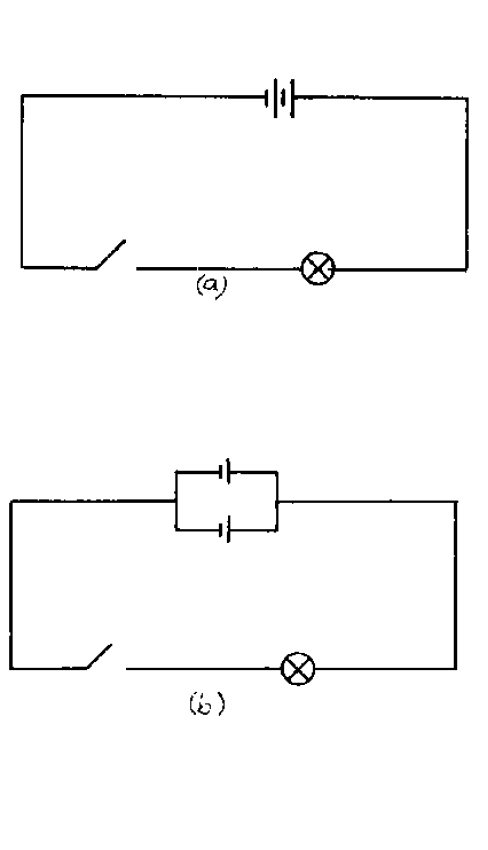
\includegraphics[width=0.3\textwidth]{./img/source/measuring-emf.png}
\end{center}

\begin{description*}
%\item[Subtopic:]{}
\item[Materials:]{Dry cell batteries, speaker wire, voltmeter/multimeter}
%\item[Setup:]{Set up the circuits shown in the figure.}
\item[Procedure:]{Connect the terminals of the multimeter to the terminals of the battery so that a voltage level is displayed. Connect two cells in series, i.e. positive terminal of one to negative terminal of the other. Then connect two cells in parallel, i.e. positive terminal of one to positive terminal of the other.}
%\item[Hazards:]{}
\item[Questions:]{What difference is there in the voltage readings?}
\item[Observations:]{The voltage level is higher when the cells are in series (around 3 V) than when in parallel (around 1.5 V)}
\item[Theory:]{The potential difference in a cell or battery when no current flows out of the battery is the \emph{electromotive force (e.m.f.)} of the cell. The voltage of two cells add together in series, but in parallel, it stays the same as that of a single cell.}
\item[Applications:]{In torches and car batteries cells are connected in series to get the required voltage. In cars, 12 volts are needed, so 6 cells are connected in series, since each cell carries only 2 V.}
%\item[Notes:]{}
\end{description*}

\vfill
\columnbreak

%==================================================================================================%

\section*{Electric Current and \hfill \\ Resistance}


\subsection{Internal Resistance of a Cell} \index{Internal resistance|see{Practicals}} \index{Practicals! internal resistance of a cell}
\textbf{*NECTA PRACTICAL*}

\begin{center}
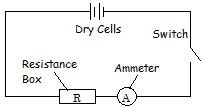
\includegraphics[width=0.4\textwidth]{./img/ohms-law.png}
\end{center}

\begin{description*}
%\item[Subtopic:]{}
\item[Materials:]{Dry cell, resistance box/rheostat, ammeter/galvanometer, speaker wire}
\item[Setup:]{Connect the circuit shown.}
\item[Procedure:]{Adjust the resistance box/rheostat to give 1 $\Omega$. Read the current $I$ on the ammeter. Repeat for different resistances (2 $\Omega$, 3 $\Omega$, 4 $\Omega$, 5 $\Omega$).}
%\item[Hazards:]{}
\item[Questions:]{Plot a graph of resistance, $R$ (vertical) against $\frac{1}{I}$ (horizontal). Find the slope and $y$-intercept.}
\item[Observations:]{According to Ohm's Law, $V = IR$. When accounting for internal resistance of a cell, this becomes, $V = I(R + r)$. Solving for $R$ we get, $R = \frac{V}{I} - r$. Because $\frac{1}{I}$ is the value on the $x$-axis, we can see that this equation follows the standard $y=mx+c$ form, where the slope $m$ in this case is the voltage $V$, and the $y$-intercept $c$ is in this case $-r$ (crosses the $y$-axis at a negative value, though $r$ itself is positive).}
\item[Theory:]{Cells have an internal resistance that opposes flow of current through them. This value can be obtained through experiment as outlined above.}
%\item[Applications:]{}
%\item[Notes:]{}
\end{description*}

\vfill
\columnbreak

\subsection[Making a Potentiometer/Metre Bridge]{Making a Potentiometer/ \hfill \\ Metre Bridge} \index{Potentiometer!NECTA practical|see{Practicals}} \index{Metre bridge!NECTA practical|see{Practicals}} \index{Potentiometer! construction of} \index{Metre bridge! construction of}

\begin{center}
%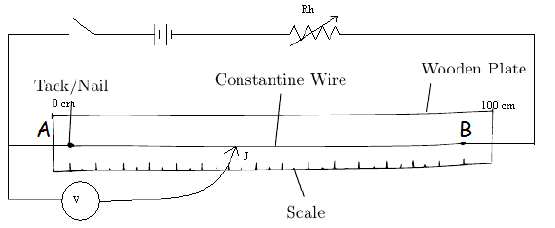
\includegraphics[width=0.4\textwidth]{./img/potentiometer.png}
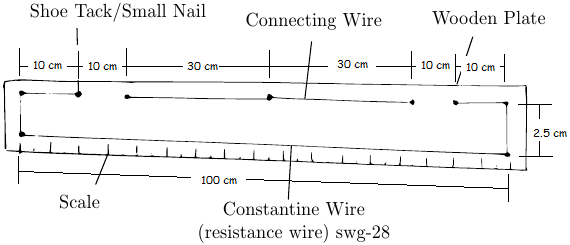
\includegraphics[width=0.49\textwidth]{./img/metre-bridge-2.png}
\end{center}

\begin{description*}
%\item[Subtopic:]{}
\item[Materials:]{Wooden plate 110 cm $\times$ 4 cm, Constantine or nichrome wire, small nails, metre rule}
%\item[Setup:]{}
\item[Procedure:]{Fix nails into the wooden plate as shown in the figure. Use a metre rule to mark a cm scale along the bottom side and fix resistance wire between the nails, making sure the wire is tight. Use connecting wire to join the other nails as shown.}
%\item[Hazards:]{}
%\item[Questions:]{}
%\item[Observations:]{}
%\item[Theory:]{}
%\item[Applications:]{}
%\item[Notes:]{}
\end{description*}

\subsection{The Potentiometer} \index{Practicals! potentiometer}
\textbf{*NECTA PRACTICAL*}

\begin{center}
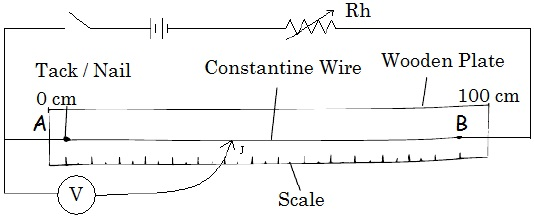
\includegraphics[width=0.45\textwidth]{./img/potentiometer.jpg}
\end{center}

\begin{description*}
%\item[Subtopic:]{}
\item[Materials:]{Potentiometer (see above), dry cells, resistance box/rheostat, voltmeter}
\item[Setup:]{Set up the circuit as shown by connecting 2 dry cells across the first gap in the potentiometer assembled above, and a rheostat across the second gap. Connect one lead of the voltmeter to one end of the resistance wire and leave the other lead free to move (J).}
\item[Procedure:]{Adjust the rheostat so that when J touches B, there is a near full deflection of the voltmeter. Now place the terminal J of the voltmeter 10 cm from side A. Record the voltage reading. Repeat for different values of AJ (20 cm, 30 cm, 50 cm, 70 cm).}
%\item[Hazards:]{}
\item[Questions:]{Tabulate your results and plot a graph of voltage (V) against AJ. Calculate the slope of the graph.}
%\item[Observations:]{The reading on the voltmeter increases as the length of AJ increases.}
\item[Theory:]{From Ohm's Law, $V = IR$. However, resistance depends on many factors, including length $l$, resistivity $\rho$, and cross-sectional area $A$. Hence this equation can be rewritten as $V = \cfrac{I \rho l}{A}$. Because we are plotting against $l$, the slope of the graph is $\cfrac{I \rho}{A}$.}
%\item[Applications:]{}
%\item[Notes:]{}
\end{description*}

\subsection{Wheatstone Bridge} \index{Practicals! metre bridge}
\textbf{*NECTA PRACTICAL*}

\begin{center}
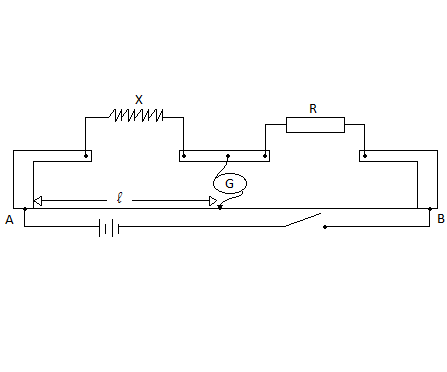
\includegraphics[width=0.49\textwidth]{./img/metre-bridge-assembly.png}
\end{center}

\begin{description*}
%\item[Subtopic:]{}
\item[Materials:]{Metre bridge (see above), dry cells, galvanometer, resistance box, unknown resistor (e.g. 10 $\Omega$)}
\item[Setup:]{Connect the circuit as shown by placing one \emph{unknown} resistor ($X$) across the first gap of the metre bridge assembled above, and a resistance box ($R$) across the second gap. Connect 2 dry cells across either end of the resistance wire and a galvanometer attached at one end with its other terminal free to move as shown.}
\item[Procedure:]{Adjust the resistance box to 1 $\Omega$ and slide the jockey, J (free lead of galvanometer) along the resistance wire until the galvanometer gives a zero reading. Record the length $l$ of AJ. Repeat for different values of the resistance box (2 $\Omega$, 4 $\Omega$, 7 $\Omega$, 10 $\Omega$).}
%\item[Hazards:]{}
\item[Questions:]{Tabulate your values and plot a graph of resistance $R$ against $\cfrac{1}{l}$. Find the slope and $y$-intercept of the graph and use them to determine the value of the unknown resistance $X$.}
%\item[Observations:]{}
\item[Theory:]{The balancing ratio for the wheatstone bridge states that $\cfrac{X}{l} = \cfrac{R}{(100-l)}$. Solving for $R$, we get $R = \cfrac{X}{l}(100-l)$, or $R = \cfrac{100X}{l}-X$. From this equation it can be seen that the slope of the graph is $100X$ and the $y$-intercept is simply the unknown resistance $X$.}
%\item[Applications:]{}
%\item[Notes:]{}
\end{description*}

\vfill
\columnbreak

%==================================================================================================%

\section*{Heat and Electric Current}


\subsection{Heating Effect of an Electric Current}

\begin{center}
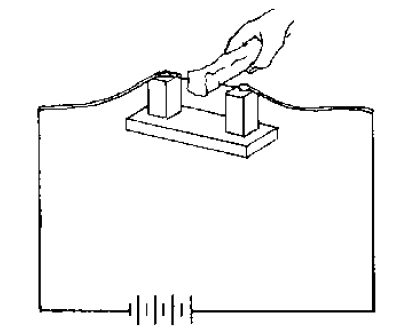
\includegraphics[width=0.4\textwidth]{./img/source/heat-current.png}
\end{center}

\begin{description*}
%\item[Subtopic:]{}
\item[Materials:]{Styrofoam, dry cells, speaker wire, steel wool, wooden blocks}
\item[Setup:]{Set up the circuit as shown by connecting a thin strand of steel wool across two wire ends supported by wooden blocks.}
\item[Procedure:]{Wait a short time for the steel wool to heat up. It may begin to glow red. Press the Styrofoam gently across the steel wool.}
\item[Hazards:]{Don't touch the heated steel wool!}
%\item[Questions:]{}
\item[Observations:]{The steel wool easily cuts through the Styrofoam.}
\item[Theory:]{The electrical energy in the circuit has been converted into heat energy which melts the Styrofoam.}
\item[Applications:]{Electric iron, electric kettle, electric cooker}
%\item[Notes:]{}
\end{description*}

\subsection{Electric Matches}

%\begin{center}
%\includegraphics[width=0.4\textwidth]{./img/source/.png}
%\end{center}

\begin{description*}
%\item[Subtopic:]{}
\item[Materials:]{Dry cells, steel wool, matches}
\item[Setup:]{Set up the circuit as above.}
\item[Procedure:]{Instead of using Styrofoam, wrap the steel wool around the head of a match and connect the circuit.}
%\item[Hazards:]{}
%\item[Questions:]{}
\item[Observations:]{The match heats up and after a short time it ignites.}
\item[Theory:]{Electric current produces heat energy which lights the match.}
%\item[Applications:]{}
%\item[Notes:]{}
\end{description*}

\columnbreak

\subsection{Making an Electric Heater} \index{Electric heater}

\begin{center}
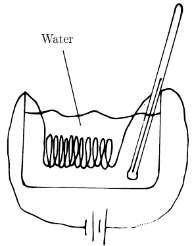
\includegraphics[width=0.2\textwidth]{./img/electric-heater.png}
\end{center}

\begin{description*}
%\item[Subtopic:]{}
\item[Materials:]{Nichrome (resistance) wire (1 m), paper, speaker wire, 2-4 dry cells, water container, thermometer (optional)}
%\item[Setup:]{}
\item[Procedure:]{Roll a piece of paper and coil the resistance wire around it so that the coils are close but not touching. Use speaker wires to connect the ends of the resistance wire to the terminals of the batteries. Place the coil of resistance wire into the container of water.}
\item[Hazards:]{Do not touch the water when current is flowing. If the heater is connected to the cells while not in the water, the wire can melt or burn other objects.}
%\item[Questions:]{}
\item[Observations:]{By touching the water container \emph{on the outside}, it begins to warm up. If left for long enough, the water will begin to boil.}
\item[Theory:]{The electric heater converts electrical energy into heat energy. The larger the coils are, the more efficient the heater will be.}
\item[Applications:]{Boiling water, heating houses}
%\item[Notes:]{}
\end{description*}

\subsection{The Fuse} \index{Fuse}

\begin{center}
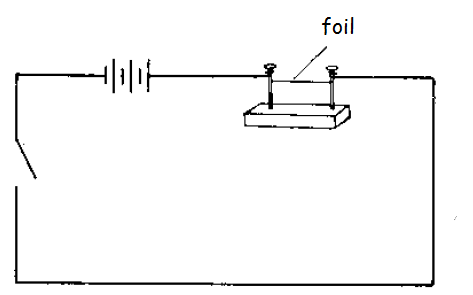
\includegraphics[width=0.3\textwidth]{./img/source/fuse.png}
\end{center}

\begin{description*}
%\item[Subtopic:]{}
\item[Materials:]{Power source, speaker wire, 2 small nails, small piece of wood, metal foil}
%\item[Setup:]{}
\item[Procedure:]{Hammer the nails into the wood about 5 cm apart. Connect wires to each nail and secure a thin strip of foil between them. Connect wires to the power source.}
%\item[Hazards:]{}
%\item[Questions:]{}
\item[Observations:]{The foil will heat and eventually burn, breaking the circuit.}
\item[Theory:]{Foil has a very small cross-sectional area compared to that of a wire, so it has a low tolerance for current. If too much current passes through the foil, it will burn away.}
\item[Applications:]{Radios or other electrical devices to prevent large currents which could start fires.}
%\item[Notes:]{}
\end{description*}

%==================================================================================================%

\section*{Cells}


\subsection{Opening a Dry Cell} \index{Dry cells}

\begin{center}
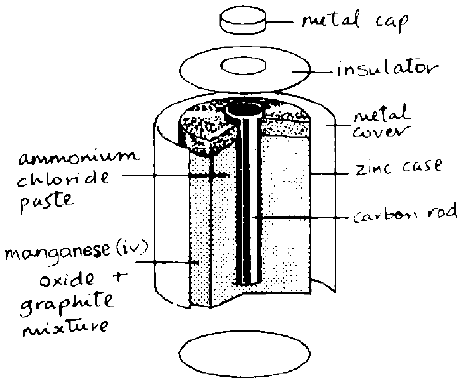
\includegraphics[width=0.49\textwidth]{./img/source/dry-cell-a.png}
\end{center}

\begin{description*}
%\item[Subtopic:]{}
\item[Materials:]{Dry cell battery, knife}
%\item[Setup:]{}
\item[Procedure:]{Remove the outer coating and cut the inside in half so the components can be seen clearly.}
\item[Hazards:]{The black powder found in the dry cell is poisonous and will also corrode metal - wash all tools well that touch the powder.}
%\item[Questions:]{}
\item[Observations:]{The black rod in the centre is a carbon rod (graphite). The black substance contains manganese (IV) oxide and ammonium chloride paste. There is a zinc plate surrounding the black powder.}
\item[Theory:]{The electrical energy is produced by a chemical reaction between the zinc and the ammonium chloride paste.}
\item[Applications:]{Zinc cases and carbon rods may be used for other activities.}
%\item[Notes:]{}
\end{description*}

\vfill
\columnbreak

\subsection{Creating a Leclanche Cell} \index{Leclanche cell}

\begin{center}
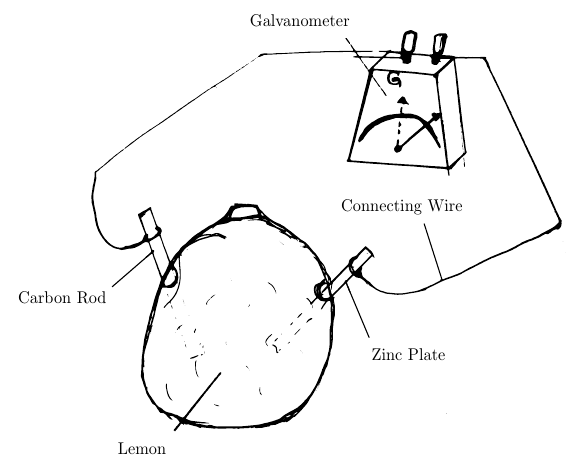
\includegraphics[width=0.45\textwidth]{./img/lechlanche-cell.png}
\end{center}

\begin{description*}
%\item[Subtopic:]{}
\item[Materials:]{Lemons, zinc plate and carbon rod from old dry cell (see above), connecting wires, galvanometer, bulb}
%\item[Setup:]{}
\item[Procedure:]{Make two holes in a lemon and insert the carbon rod and zinc plate into the holes. Connect the lemon to the galvanometer using connecting wires and notice any deflection that may occur. Repeat for several lemons by placing them in series and in parallel.}
%\item[Hazards:]{}
%\item[Questions:]{}
\item[Observations:]{The deflection increases with the number of lemons placed in series. With enough lemons, the bulb will light up.}
\item[Theory:]{Electric current can be produced from different cells - dry and wet. Wet cells can be made from natural foods such as lemons, Irish potatoes and salts which produce electric current based on the principle of Leclanche cells.}
%\item[Applications:]{}
%\item[Notes:]{}
\end{description*}






\end{multicols}

\pagebreak